\documentclass{scrartcl}

\usepackage{amssymb}
\usepackage{amsmath}
\usepackage{tikz}
\usetikzlibrary{decorations, arrows, arrows.meta}

%Deleuze & Guattari - A Thousand Plateaus, pp. 135 & 137

\begin{document}
	
	\hspace{2.5cm}
	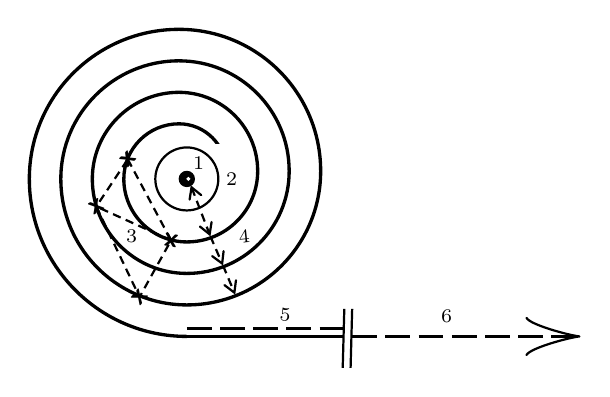
\begin{tikzpicture}
	\path [very thick, draw=black, postaction=decorate]
	(180:2) \foreach \a in {-5,...,12}{ arc (180-\a*90:90-\a*90:1.5-\a/10) };
	
	%circles inside spiral
	\fill[white] (-2.5,1.5) rectangle (-1.4,2.45);
	\draw[thick] (-2,2) circle (0.4cm);
	\node[circle,draw=black, fill=black, inner sep=0pt,minimum size=5.5pt] at (-2,2) {};
	\node[circle,draw=white, fill=white, inner sep=0pt,minimum size=1pt] at (-1.98,2) {};
	
	%arrows inside spiral
	\draw[<->,>=angle 60,thick,densely dashed] (-1.95,1.92)--(-1.7,1.27);
	\draw[->,>=angle 60,thick,densely dashed] (-1.7,1.27)--(-1.54,0.9);
	\draw[->,>=angle 60,thick,densely dashed] (-1.54,0.9)--(-1.385,0.53);
	
	%x's
	\node at (-2.75,2.25){\rotatebox{45}{\textbf{\textsf{x}}}};		%topmost
	\node at (-2.2,1.22) {\rotatebox{170}{\textbf{\textsf{x}}}};	%rightmost
	\node at (-3.15,1.65){\rotatebox{30}{\textbf{\textsf{x}}}};		%leftmost
	\node at (-2.6,0.5)  {\rotatebox{50}{\textbf{\textsf{x}}}};		%bottom
	\draw[thick,densely dashed] (-2.75,2.25)--(-2.2,1.22)--(-2.6,0.5)--(-3.15,1.65)--(-2.75,2.25);
	\draw[thick,densely dashed] (-2.2,1.22)--(-3.15,1.65);
	
	%end of spiral
	\draw[line width=0.9pt,dash pattern=on 9pt off 3pt] (-2,0.1)--(0,0.1);
	\draw[line width=1pt] (-2,0)--(0,0);
	
	%vertical lines
	\draw[thick] (0,0.35)--(-0.02,-0.4);
	\draw[thick] (0.1,0.35)--(0.08,-0.4);
	
	\draw[-{Classical TikZ Rightarrow[length=7mm,width=5mm]},line width=1pt,dash pattern=on 9pt off 3pt] (0.1,0)--(3,0);
	
	%numbers
	\node at (-1.85,2.2) {{\scriptsize 1}};
	\node at (-1.43,2)	 {{\scriptsize 2}};
	\node at (-2.7,1.27) {{\scriptsize 3}};
	\node at (-1.27,1.27){\rotatebox{6}{\scriptsize 4}};
	\node at (-0.75,0.27){\rotatebox{-6}{\scriptsize 5}};
	\node at (1.3,0.25)  {{\scriptsize 6}};
	
	%\draw[help lines] (-4,0) grid (3,4);
	\end{tikzpicture}
	
	\vspace{0.4cm}
	
	{\small\hspace{-1.4cm}(1) The point of subjectification, replacing the center of signifiance.}
	
	{\small\hspace{-1.4cm}(2) The two faces turned away from each other.}
	
	{\small\hspace{-1.4cm}(3) The subject of enunciation resulting from the point of subjectification and the turning away.}
	
	{\small\hspace{-1.4cm}(4) The subject of the statement, into which the subject of enunciation recoils.}
	
	{\small\hspace{-1.4cm}(5) \hspace{0.03cm}The succession of finite linear proceedings accompanied by a new form of priest \& a new bureaucracy.}
	
	{\small\hspace{-1.4cm}(6) The line of flight, which is freed but still segmented, remaining negative and blocked.}
	
	
	\vspace{1.5cm}
	
	
	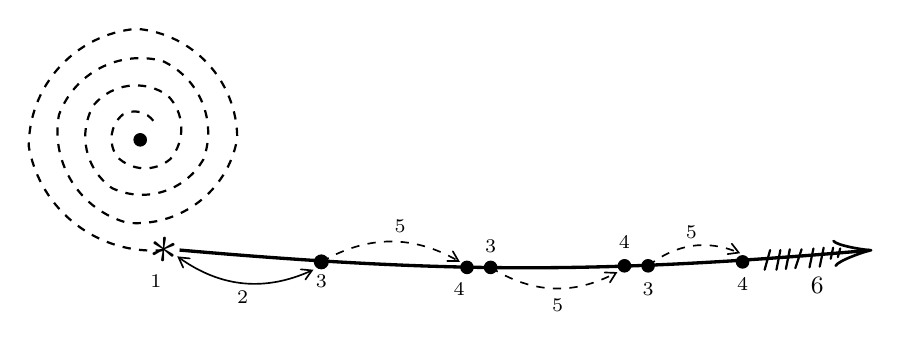
\begin{tikzpicture}
	%spiral
	\path [thick, draw=black, postaction=decorate,dashed]
	(180:2) \foreach \a in {-1,...,12}{ arc (180-\a*95:95-\a*95:1.5-\a/10) };	%↑ing to 95 makes it choppier
	%
	\node[circle,draw=black, fill=black, inner sep=0pt,minimum size=4.5pt] at (-2.3,1.4) {};
	\node at (-2,0) {\rotatebox{-5}{\huge$\ast$}};
	
	%main arrows
	\draw[-{Classical TikZ Rightarrow[length=5mm,width=3.5mm]},very thick] (-1.8,0) to[out=-5,in=185] (7,0);
	\node[circle,draw=black, fill=black, inner sep=0pt,minimum size=5pt] at (0,-0.15) {};
	\node[circle,draw=black, fill=black, inner sep=0pt,minimum size=4.5pt] at (1.85,-0.22) {};
	\node[circle,draw=black, fill=black, inner sep=0pt,minimum size=4.5pt] at (2.15,-0.22) {};
	\node[circle,draw=black, fill=black, inner sep=0pt,minimum size=4.5pt] at (3.85,-0.2) {};
	\node[circle,draw=black, fill=black, inner sep=0pt,minimum size=4.5pt] at (4.15,-0.2) {};
	\node[circle,draw=black, fill=black, inner sep=0pt,minimum size=4.5pt] at (5.35,-0.15) {};
	
	%small arrows
	\draw[<->,>=angle 60,semithick] (-1.83,-0.08) to[bend right] (-0.1,-0.25);
	\draw[->,>=angle 60,semithick,dashed] (0,-0.15) to[bend left] (1.76,-0.15);
	\draw[->,>=angle 60,semithick,dashed] (2.15,-0.22) to[bend right] (3.76,-0.28);
	\draw[->,>=angle 60,semithick,dashed] (4.15,-0.2) to[bend left] (5.32,-0.04);
	
	%diagonal lines
	\draw[thick,line cap=round] (5.7,0)--(5.63,-0.25);
	\draw[thick,line cap=round] (5.83,0)--(5.78,-0.25);
	\draw[thick,line cap=round] (5.95,0.01)--(5.9,-0.24);
	\draw[thick,line cap=round] (6.1,0.01)--(6.02,-0.23);
	\draw[thick,line cap=round] (6.25,0.02)--(6.2,-0.22);
	\draw[thick,line cap=round] (6.38,0.03)--(6.33,-0.21);
	\draw[thick,line cap=round] (6.5,0.03)--(6.47,-0.11);
	\draw[thick,line cap=round] (6.59,0.02)--(6.56,-0.09);
	
	%labels
	\node at (-2.1,-0.4) {{\scriptsize 1}};
	\node at (-1,-0.6) 	 {{\scriptsize 2}};
	\node at (0,-0.4) 	 {{\scriptsize 3}};
	\node at (1,0.3) 	 {{\scriptsize 5}};
	\node at (1.75,-0.5) {{\scriptsize 4}};
	\node at (2.15,0.05) {{\scriptsize 3}};
	\node at (3,-0.7) 	 {{\scriptsize 5}};
	\node at (3.85,0.1)  {{\scriptsize 4}};
	\node at (4.15,-0.5) {{\scriptsize 3}};
	\node at (4.7,0.22)  {{\scriptsize 5}};
	\node at (5.35,-.43) {{\scriptsize 4}};
	\node at (6.3,-0.45) {{\small 6}};
	
	%\draw[help lines] (-4,-1) grid (7,3);
	\end{tikzpicture}
	
	\vspace{0.25cm}
	
	{\small\hspace{-1.4cm}(1) The Center or the Signifier; the faciality of the god or despot.}
	
	{\small\hspace{-1.4cm}(2) The Temple or Palace, with priests and bureaucrats.}
	
	{\small\hspace{-1.4cm}(3) \hspace{0.03cm}The organization in circles \& the sign referring to other signs on the same circle or on different$\;$circles.}
	
	{\small\hspace{-1.4cm}(4) The interpretive development of signifier into signified, which then reimparts signifier.}
	
	{\small\hspace{-1.4cm}(5) The expiatory animal; the blocking of the line of flight.}
	
	{\small\hspace{-1.4cm}(6) The scapegoat, or the negative sign of the line of flight.}
\end{document}